\documentclass[a4paper,11pt]{scrartcl}
\usepackage{graphicx}
\usepackage[utf8]{inputenc}
\usepackage[T1]{fontenc}
\usepackage[ngerman]{babel}
\usepackage{bibgerm}
\usepackage{amsmath,amssymb,amsthm}
\usepackage{color}
\usepackage{enumerate}
\usepackage{tabularx}
\usepackage{subfig}
\usepackage{fancyhdr}
\usepackage{upgreek}
\usepackage{graphicx}
\usepackage{framed}
\usepackage{lmodern}
\usepackage{geometry}
\geometry{a4paper,left=2.5cm,right=1.5cm, top=1cm, bottom=2cm} 
\usepackage{marginnote}
\usepackage[pdftex,pdfpagelabels,colorlinks,backref,pagebackref,plainpages=false]{hyperref}
\setlength{\headwidth}{15cm}
\setlength{\textwidth}{15cm}

\usepackage{shadethm}
% == Set the heading style ===================================================
\setlength{\headheight}{14pt}
%\pagestyle{fancyplain}
\renewcommand{\sectionmark}[1]{\markboth{#1}{}}
\renewcommand{\subsectionmark}[1]{\markright{\thesection\ #1}}
\lhead[\fancyplain{}{\thepage}]{\fancyplain{}{\rightmark}}
\rhead[\fancyplain{}{\leftmark}]{\fancyplain{}{\thepage}}
\cfoot{}
\renewcommand{\headrulewidth}{0.4pt}
% ============================================================================

% == Set correct values for fitting floats ===================================
\tolerance=2000
\emergencystretch=10pt

\setcounter{topnumber}{3}
\setcounter{totalnumber}{5}
\setcounter{bottomnumber}{2}

% To make those darn floats fit where they should
\setcounter{totalnumber}{9}
\setcounter{topnumber}{9}
\setcounter{bottomnumber}{9}
\renewcommand{\textfraction}{0.00}
\renewcommand{\topfraction}{1.0}
\renewcommand{\bottomfraction}{1.0}
% ============================================================================

% == Abkürzungen für die reellen, natürlichen, ganzen,... Zahlen =============
\newcommand{\R}{{\ensuremath{\mathbb{R}}}}
\newcommand{\N}{{\ensuremath{\mathbb{N}}}}
\newcommand{\Z}{{\ensuremath{\mathbb{Z}}}}
\newcommand{\C}{{\ensuremath{\mathbb{C}}}}
\newcommand{\Q}{{\ensuremath{\mathbb{Q}}}}
\newcommand{\F}{{\ensuremath{\mathbb{F}}}}
\newcommand{\Prim}{{\ensuremath{\mathbb{P}}}}
% ============================================================================

\newcommand{\RM}[1]{\MakeUppercase{\romannumeral #1{}}} 

% == Makros für Autorenname und -adresse =====================================
\newcommand{\myaddress}[6]{%
  \parbox{\textwidth}{\textbf{\large #1}\\
    #2\\ #3\\ #4\\ 
    \ifthenelse{\equal{#5}{}}{}{Email: \href{mailto:#5}{\texttt{#5}}\\}
    \ifthenelse{\equal{#6}{}}{}{WWW: \href{#6}{\path|#6|}\\}
  } 
}

\newcommand{\myauthor}[1]{%
  \addtocontents{toc}{\protect\hspace{3.35ex}%
  \textsl{#1}\par}\vspace{-4ex}\quad\hfill\textsl{\Large #1}\vspace{8ex}}

\newcommand{\myname}[1]{\Large #1}

%%%%%%%%%%%%%%%%%%%%%%%%%%%%%%%%%%%%%%%%%%%%%%%%%%
% Tragen Sie in der folg. Zeile Ihren Namen ein: %
%%%%%%%%%%%%%%%%%%%%%%%%%%%%%%%%%%%%%%%%%%%%%%%%%%

\newcommand{\OO}{{\ensuremath{\mathcal{O}}}}
\newcommand{\const}{\ensuremath{\equiv}}

%\renewcommand{\thechapter}{\Roman{chapter}}
\renewcommand{\thesection}{\arabic{section}}


\newenvironment{Kasten}[1]
{
\hspace{0.05\linewidth}
\begin{center}
\begin{minipage}{0.95\linewidth}
\setlength{\fboxsep}{10pt}
%\setlength{\fboxsep}{18pt}
%\definecolor{shadecolor}{gray}{0.9}
\definecolor{shadecolor}{rgb}{0.9,1,1}
\definecolor{framecolor}{gray}{0}
%\def\FrameCommand{\fcolorbox{framecolor}{shadecolor}}
%\MakeFramed {\FrameRestore}
\subsubsection*{#1}
%\begin{itshape}
}
{
%\end{itshape}
%\endMakeFramed
\end{minipage}
\end{center}
%\vspace{1em}
}


\newenvironment{bsp}[1]
{
\setlength{\fboxsep}{10pt}
\subsection*{Beispiel: #1}
\begin{upshape}
}
{
\end{upshape}
}


\newenvironment{definition}[1]{
	\begin{definitions}
	\marginnote{\emph{#1}}
}{\end{definitions}}


\begin{document}
\pagestyle{empty}
\author{\large Simon Bischof}
\title{{\LARGE $n$-dimensionale Polarkoordinaten} \\ {\large Zusammenfassung}}
\date{}
\maketitle
\shorthandoff{"}
\section{Grundlegendes}
Es sei $|M|:=\int\limits_M 1dx \qquad (x\in\R^n,M\subseteq \R^n)$ der Inhalt von $M$.\\
Substitutionsregel:
\begin{equation*}
\label{subst}
\int\limits_{g(A)}f(v)dv=\int\limits_A f(u)|\det(J_g(u))| du, \qquad g:A\to g(A) \text{injektiv.}
\end{equation*}
Im Folgenden sei stets $n\in\N\setminus\{1\}$, $e_n=(0,\ldots,0,1)^T$ und $||\bullet||$ die euklidische Norm.\\
Es sei $D(R)^n:=\{(x_1,\cdots,x_n)\in\R^n|x_1^2+\cdots+x_n^2\leq R^2\}$ die $n$-dimensionale Kugel mit Radius $R$.
\section{$P_n$: Definition und Eigenschaften}
\subsection{Definition}
Es ist $P_2:[0, \infty)\times [0, 2\pi]\to \R^2$ mit $P_2(r,\varphi_1)=\begin{pmatrix}
r\cos\varphi_1\\ r\sin\varphi_1\end{pmatrix}$.\\
Für $n>2$ ist $P_n:[0,\infty)\times[0, 2\pi]\times[-\frac{\pi}{2},+\frac{\pi}{2}]^{n-2}\to \R^n$ induktiv definiert:\\[0.5em]
$P_n(r,\varphi_1, \varphi_2, \ldots, \varphi_{n-1})=\begin{pmatrix}
P_{n-1}(r,\varphi_1,\cdots,\varphi_{n-2})\cdot\cos\varphi_{n-1} \\ r\cdot\sin \varphi_{n-1}\end{pmatrix}
$ \\ $= \cos\varphi_{n-1}\begin{pmatrix}P_{n-1}(r,\varphi_1,\cdots,\varphi_{n-2}) \\ 0 \end{pmatrix}+r\sin\varphi_{n-1}e_n$\\
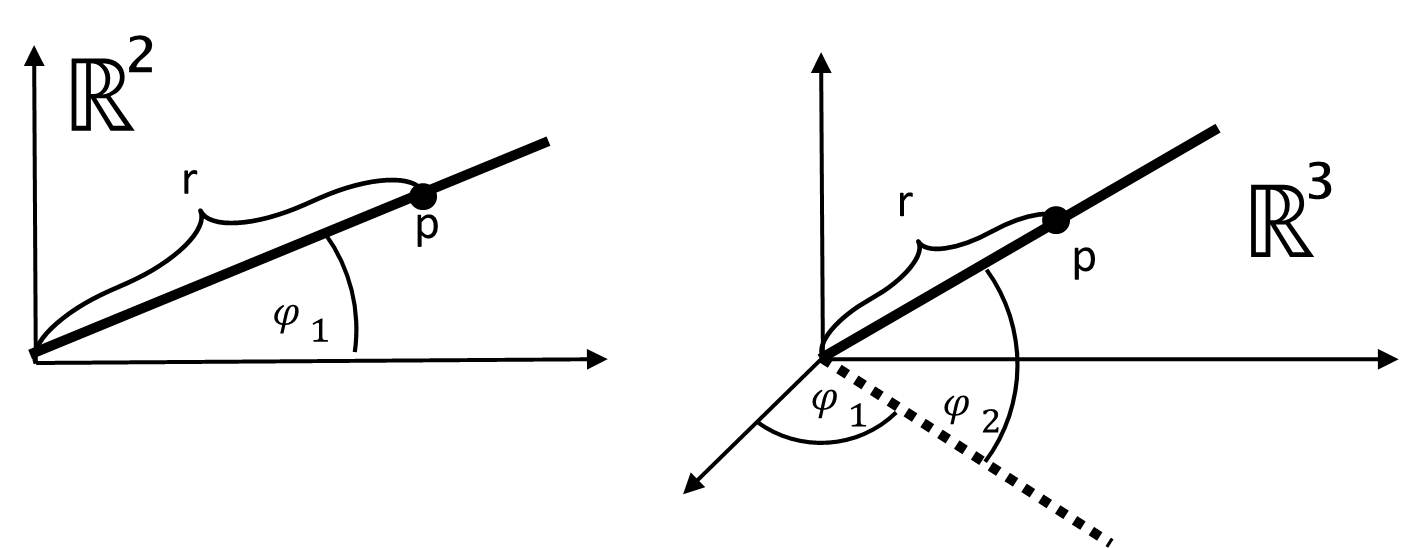
\includegraphics[scale=0.3]{images/PolarKugelkoordinaten.jpg}\\
Ausgeschrieben ergibt sich:\\
$P_n(r,\varphi_1, \varphi_2, \ldots, \varphi_{n-1})= \begin{pmatrix}r\cos\varphi_1\cos\varphi_2\cdot\ldots\cdot\cos\varphi_{n-1} \\ r\sin\varphi_1\cos\varphi_2\cdot\ldots\cdot\cos\varphi_{n-1} \\
r\sin\varphi_2\cos\varphi_3\cdot\ldots\cdot\cos\varphi_{n-1} \\
\vdots \\
r\sin\varphi_{n-2}\cos\varphi_{n-1} \\
r \sin\varphi_{n-1}
\end{pmatrix}$\\
Im Falle $n=3$ ergeben sich die bekannten Kugelkoordinaten
$$P_3(r,\varphi_1, \varphi_2)=
\begin{pmatrix}r\cos\varphi_1\cos\varphi_2 \\
r\sin\varphi_1\cos\varphi_2\\
r\sin\varphi_2\\ \end{pmatrix}$$

\subsection{$||P_n(r,\varphi_1,\cdots,\varphi_{n-1})||$}
Für $n=2: ||P_2(r,\varphi_1)||^2=r^2$, wegen $r\geq 0$ gilt also $||P_2(r,\varphi_1)||=r$.\\
Mit dem Satz des Pythagoras folgt:\\
$||P_{n+1}(r,\varphi_1,\ldots,\varphi_n)||^2=\cos^2\varphi_n\cdot||P_n(r,\varphi_1,\ldots,\varphi_{n-1})||^2 +\sin^2\varphi_n\cdot||r\cdot e_{n+1}||^2=r^2$, also $||P_{n+1}(r,\varphi_1,\ldots,\varphi_n)||=r.$

\subsection{Funktionalmatrix und -determinante}
Es ist $J_{P_2}(r,\varphi_1)=\begin{pmatrix}\cos\varphi_1 & -r\sin\varphi_1 \\
\sin\varphi_1 & r\cos\varphi_1\end{pmatrix}$ und 
$\det (J_{P_2}(r,\varphi_1))=r.$\\
Außerdem ist $J_{P_3}(r, \varphi_1, \varphi_2 )=
\begin{pmatrix} \cos\varphi_1\cos\varphi_2 & -r\sin\varphi_1\cos\varphi_2 & -r\cos\varphi_1\sin\varphi_2 \\ 
\sin\varphi_1\cos\varphi_2 & r\cos\varphi_1\cos\varphi_2 & -r\sin\varphi_1\sin\varphi_2\end{pmatrix}$ und $\det(J_{P_3}(r, \varphi_1, \varphi_2 ))=r^2\cos\varphi_2.$\\
Für allgemeines $n$ sind die Spalten der Funktionalmatrix:\\
$ \partial_r P_{n+1}(r,\varphi_1,\ldots,\varphi_n)= \begin{pmatrix}\partial_r P_n(r,\varphi_1,\ldots,\varphi_{n-1})\cdot\cos\varphi_n \\ \sin\varphi_n \end{pmatrix} $\\[1em]
$ \partial_{\varphi_k}P_{n+1}(r,\varphi_1,\ldots,\varphi_n) = \begin{pmatrix}\partial_{\varphi_k} P_n(r,\varphi_1,\ldots,\varphi_{n-1})\cdot\cos\varphi_n \\ 0 \end{pmatrix} \qquad (k=1,\ldots,n-1)$\\[1em]
$ \partial_{\varphi_n}P_{n+1}(r,\varphi_1,\ldots,\varphi_n)= \begin{pmatrix}-P_n(r,\varphi_1,\ldots,\varphi_{n-1})\cdot\sin\varphi_n \\ r\cos\varphi_n \end{pmatrix} $\\[1em]
Es ist nun
\begin{equation*}
\label{det}\det(J_{P_{n+1}}(r,\varphi_1,\ldots,\varphi_n))=\det(J_{P_n}(r,\varphi_1,\ldots,\varphi_{n-1}))\cdot r\cos^{n-1}\varphi_n.
\end{equation*}
Damit und mit $\det(J_{P_2}(r, \varphi_1))=r$ folgt rekursiv:\\
$\det(J_{P_n}(r,\varphi_1,\ldots,\varphi_{n-1}))=|\det(J_{P_n}(r,\varphi_1,\ldots,\varphi_{n-1}))|=r^{n-1}\prod\limits_{i=2}^{n-1}\cos^{i-1}\varphi_i$.
\section{Inhalt der $n$-dimensionalen Kugel}
Sei $A:=[0,R]\times[0,2\pi]\times[-\frac{\pi}{2},+\frac{\pi}{2}]^{n-2}$. Dann ist $P_n(A)=D(R)^n$.
Mit Substitutionsregel:$$\int\limits_{D(R)^n}dx=\int\limits_A |\det(J_{P_n}(r,\varphi_1,\ldots,\varphi_{n-1}))|d(r,\varphi_1,\ldots,\varphi_{n-1})\\$$
$$= \int\limits_0^R r^{n-1}dr \cdot\int\limits_0^{2\pi}d\varphi_1 \cdot\prod\limits_{i=2}^{n-1}\left(\int\limits_{-\frac{\pi}{2}}^\frac{\pi}{2}\cos^{i-1}\varphi_i d\varphi_i\right)$$\\ Es ist $|D(R)^2|=\pi R^2$, $|D(R)^3|=\frac{4\pi}{3} R^3$ und
$$|D(R)^n|=\begin{cases}\frac{\pi^q R^{2q}}{q!}; \qquad n=2q, q\in\N \\ \frac{2^{q+1}\sqrt{\pi}^q R^{2q+1}}{1\cdot 3\cdot \ldots\cdot (2q+1)} \qquad n=2q+1, q\in\N\end{cases} $$
\section{Quellen}
\begin{itemize}
\item Königsberger, Analysis 2 (S. 18f, 91f, 225-227, 287f)
\item HM-Vorlesung von Herrn Dr. Herzog (WS 2010/11, SS 2011)
\end{itemize}
\section{Materialien zum Vortrag}
Handout und Ausarbeitung finden sich jeweils als *.tex und *.pdf unter\\ \underline{https://github.com/ratefuchs/Proseminar\_Mathematik}.
\end{document}